
\begin{figure}
\centering
\begin{subfigure}{.5\textwidth}
  \centering
  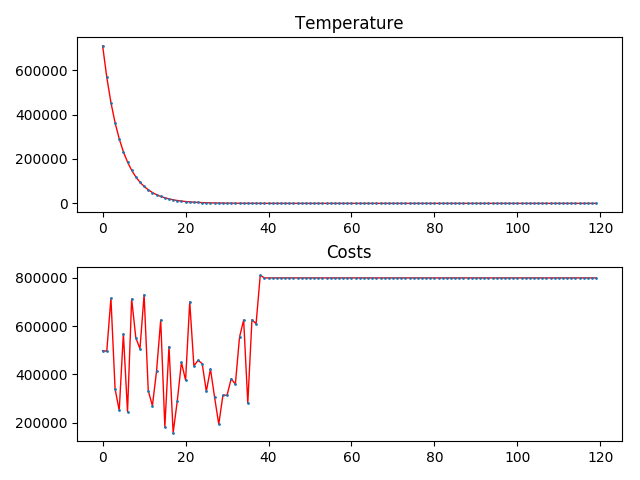
\includegraphics[width=1\linewidth]{results/cut12/1/plot}
  \label{fig:sub1}
\end{subfigure}%
\begin{subfigure}{.5\textwidth}
  \centering
  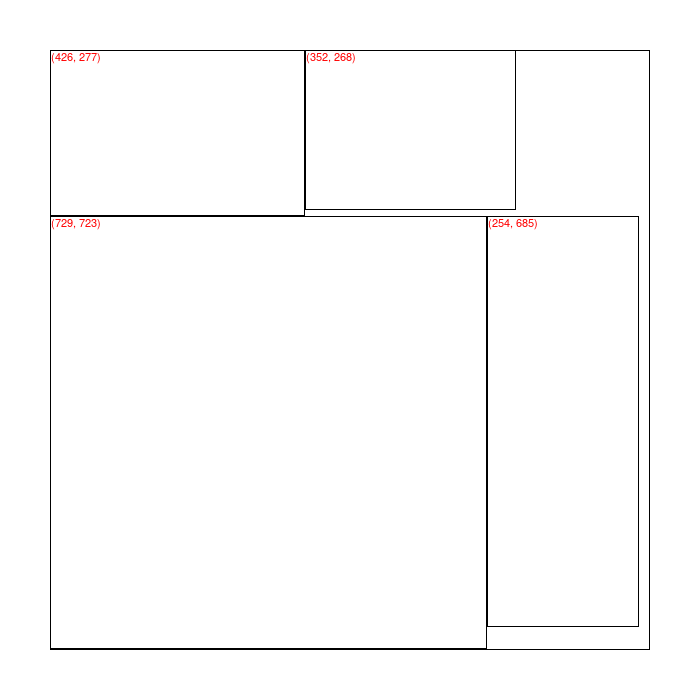
\includegraphics[width=1\linewidth]{results/cut12/1/cut}
  \label{fig:sub2}
\end{subfigure}
\caption{Instancia cut12.txt, Solução: 919054, disperdício de 8.09\% de 1000x1000}
\label{fig:test}
\end{figure}


\begin{figure}
\centering
\begin{subfigure}{.5\textwidth}
  \centering
  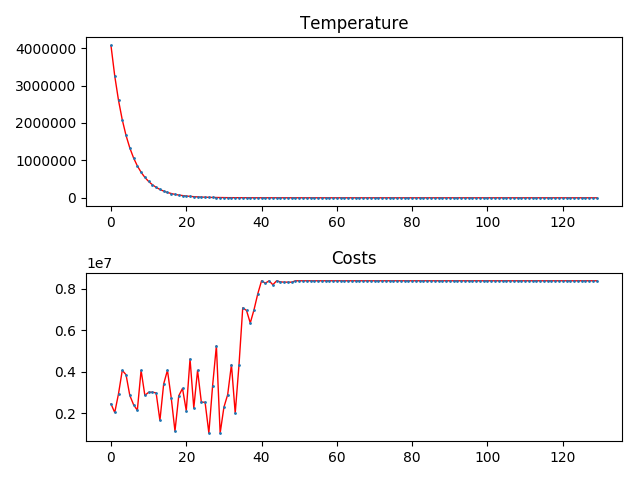
\includegraphics[width=1\linewidth]{results/cut13/1/plot}
  \label{fig:sub1}
\end{subfigure}%
\begin{subfigure}{.5\textwidth}
  \centering
  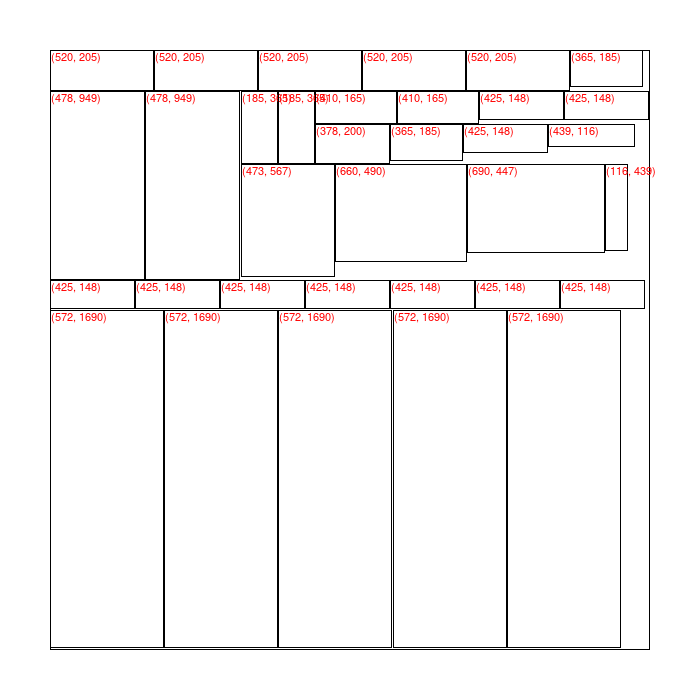
\includegraphics[width=1\linewidth]{results/cut13/1/cut}
  \label{fig:sub2}
\end{subfigure}
\caption{Instancia cut13.txt, Solução: 8344048, disperdício de 7.29\% de 3000x3000}
\label{fig:test}
\end{figure}


\begin{figure}
\centering
\begin{subfigure}{.5\textwidth}
  \centering
  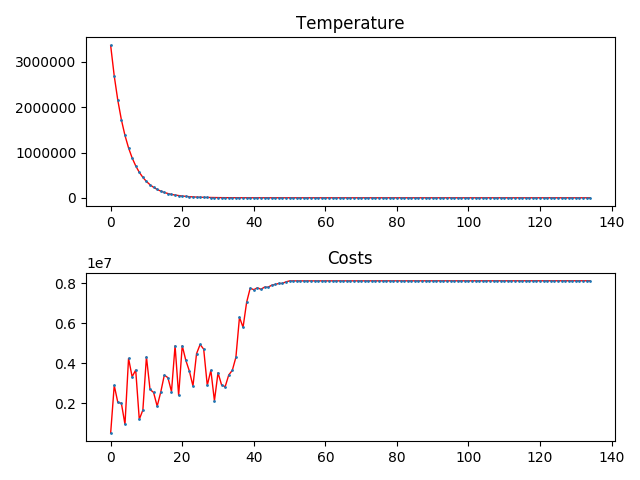
\includegraphics[width=1\linewidth]{results/cut14/1/plot}
  \label{fig:sub1}
\end{subfigure}%
\begin{subfigure}{.5\textwidth}
  \centering
  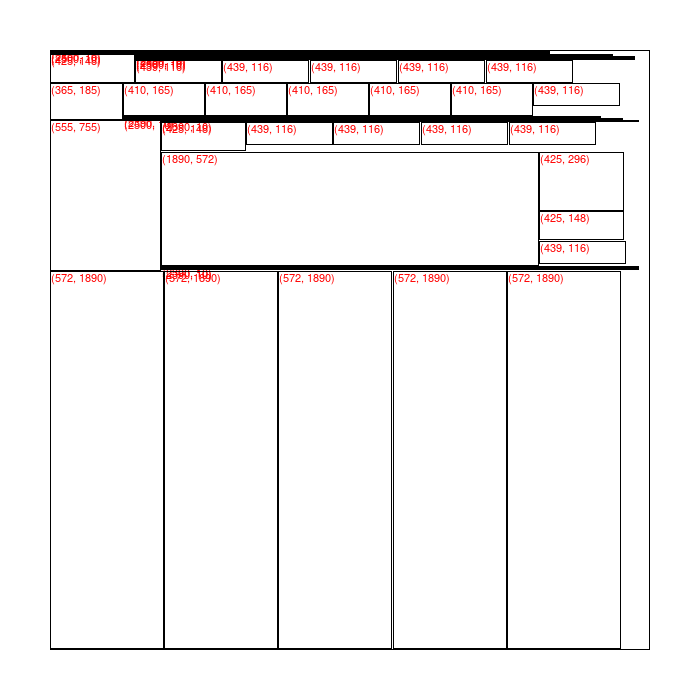
\includegraphics[width=1\linewidth]{results/cut14/1/cut}
  \label{fig:sub2}
\end{subfigure}
\caption{Instancia cut14.txt, Solução: 8430444, disperdício de 6.33\% de 3000x3000}
\label{fig:test}
\end{figure}


\begin{figure}
\centering
\begin{subfigure}{.5\textwidth}
  \centering
  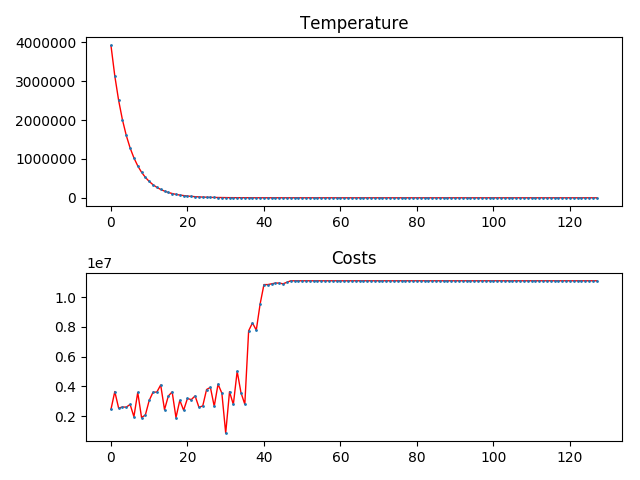
\includegraphics[width=1\linewidth]{results/cut17/2/plot}
  \label{fig:sub1}
\end{subfigure}%
\begin{subfigure}{.5\textwidth}
  \centering
  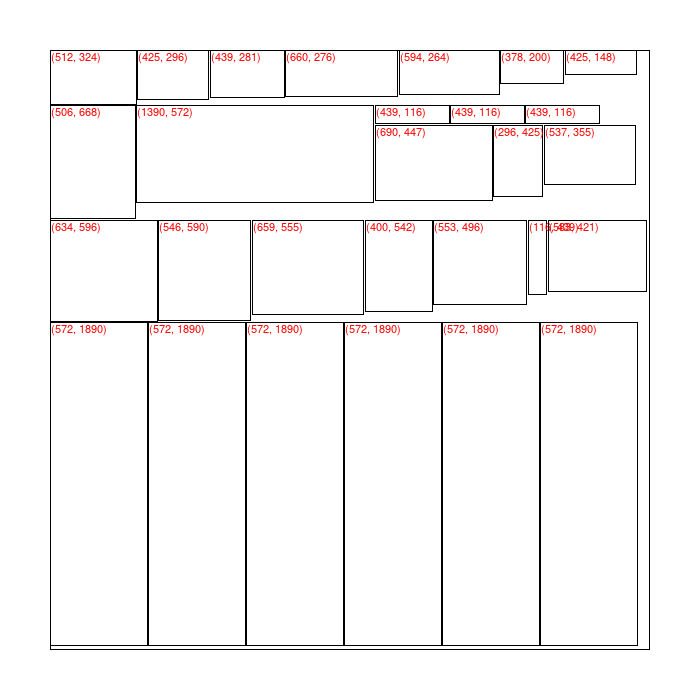
\includegraphics[width=1\linewidth]{results/cut17/2/cut}
  \label{fig:sub2}
\end{subfigure}
\caption{Instancia cut17.txt, Solução: 11175880, disperdício de 8.77\% de 3500x3500}
\label{fig:test}
\end{figure}


\begin{figure}
\centering
\begin{subfigure}{.5\textwidth}
  \centering
  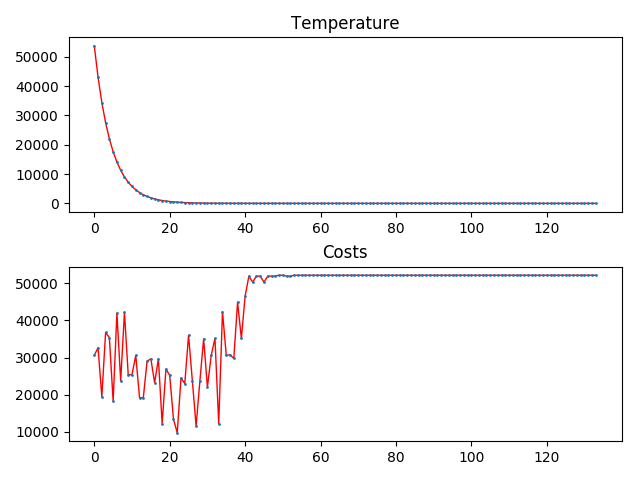
\includegraphics[width=1\linewidth]{results/cut1/3/plot}
  \label{fig:sub1}
\end{subfigure}%
\begin{subfigure}{.5\textwidth}
  \centering
  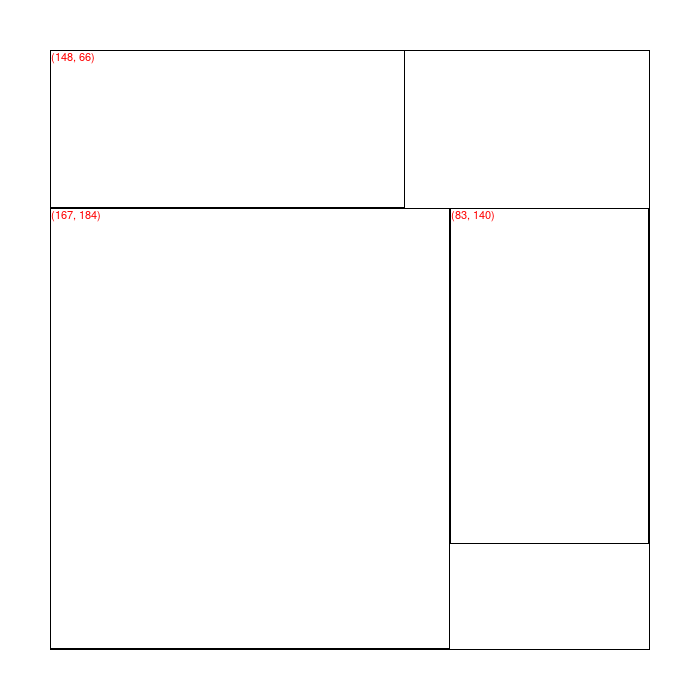
\includegraphics[width=1\linewidth]{results/cut1/3/cut}
  \label{fig:sub2}
\end{subfigure}
\caption{Instancia cut1.txt, Solução: 58136, disperdício de 6.98\% de 250x250}
\label{fig:test}
\end{figure}


\begin{figure}
\centering
\begin{subfigure}{.5\textwidth}
  \centering
  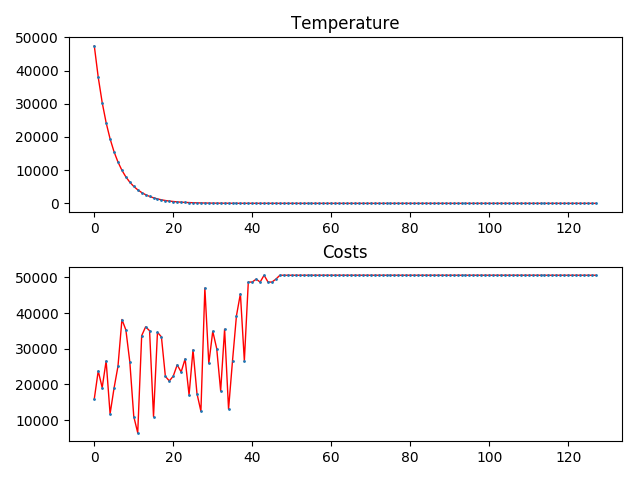
\includegraphics[width=1\linewidth]{results/cut2/3/plot}
  \label{fig:sub1}
\end{subfigure}%
\begin{subfigure}{.5\textwidth}
  \centering
  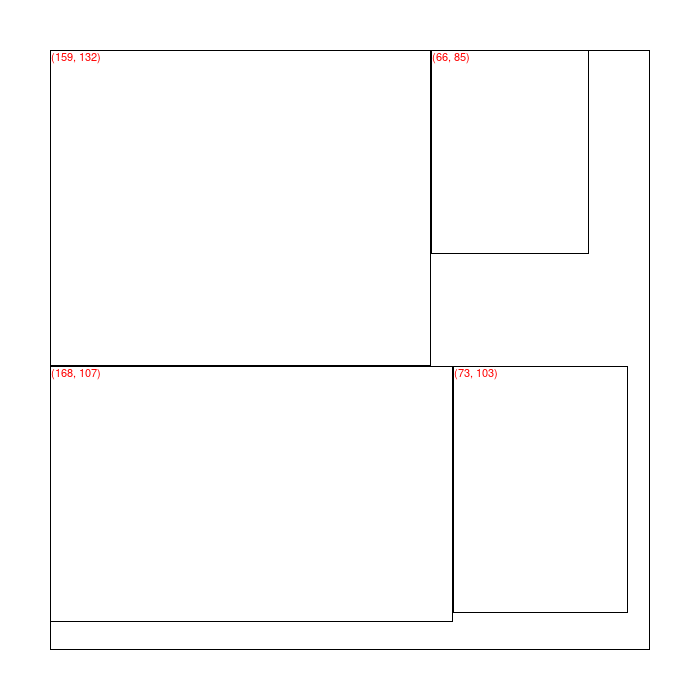
\includegraphics[width=1\linewidth]{results/cut2/3/cut}
  \label{fig:sub2}
\end{subfigure}
\caption{Instancia cut2.txt, Solução: 54002, disperdício de 13.60\% de 250x250}
\label{fig:test}
\end{figure}


\begin{figure}
\centering
\begin{subfigure}{.5\textwidth}
  \centering
  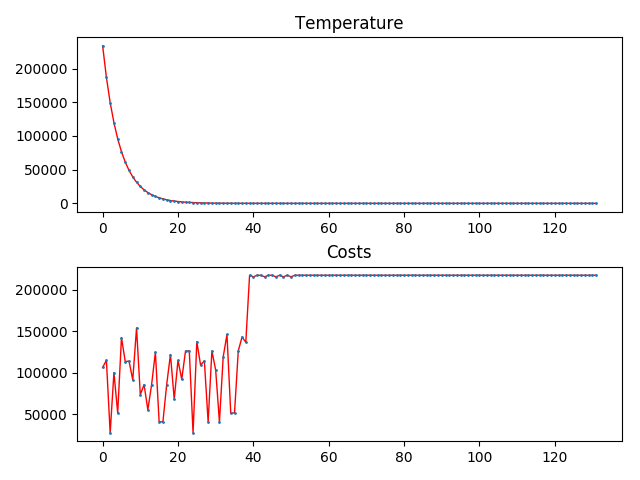
\includegraphics[width=1\linewidth]{results/cut5/1/plot}
  \label{fig:sub1}
\end{subfigure}%
\begin{subfigure}{.5\textwidth}
  \centering
  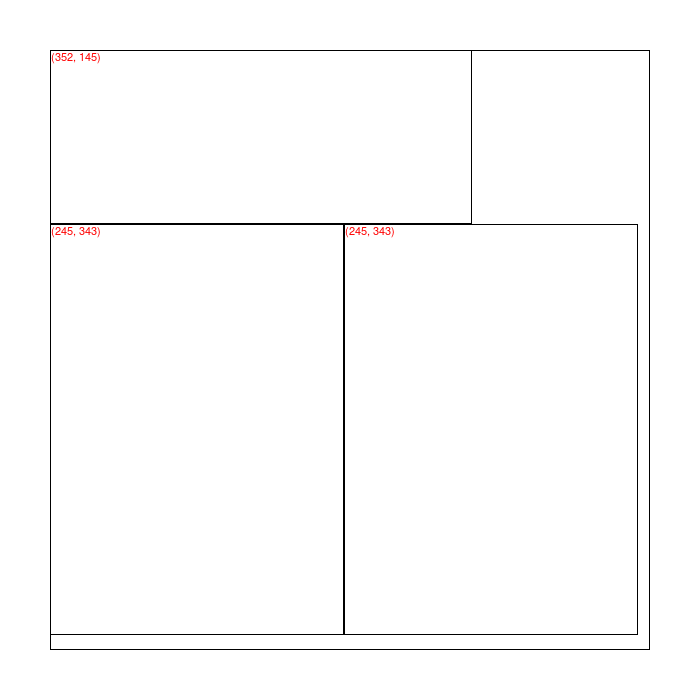
\includegraphics[width=1\linewidth]{results/cut5/1/cut}
  \label{fig:sub2}
\end{subfigure}
\caption{Instancia cut5.txt, Solução: 223560, disperdício de 10.58\% de 500x500}
\label{fig:test}
\end{figure}


\begin{figure}
\centering
\begin{subfigure}{.5\textwidth}
  \centering
  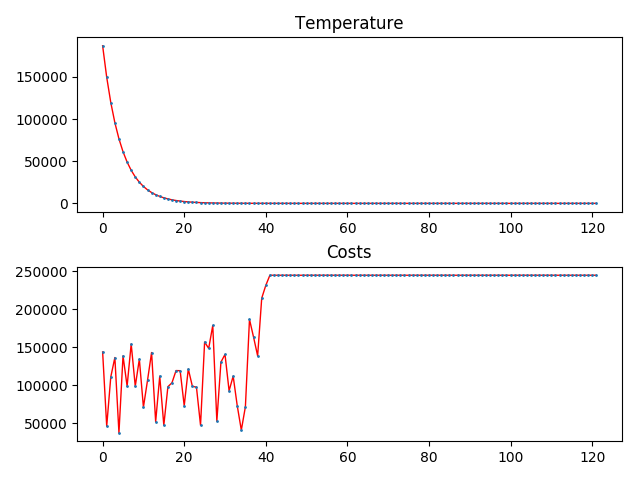
\includegraphics[width=1\linewidth]{results/cut7/1/plot}
  \label{fig:sub1}
\end{subfigure}%
\begin{subfigure}{.5\textwidth}
  \centering
  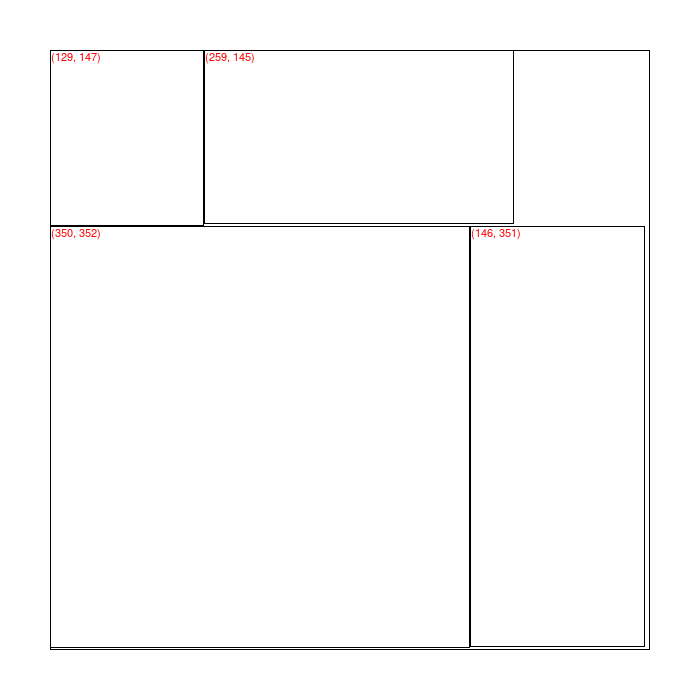
\includegraphics[width=1\linewidth]{results/cut7/1/cut}
  \label{fig:sub2}
\end{subfigure}
\caption{Instancia cut7.txt, Solução: 230964, disperdício de 7.61\% de 500x500}
\label{fig:test}
\end{figure}


\begin{figure}
\centering
\begin{subfigure}{.5\textwidth}
  \centering
  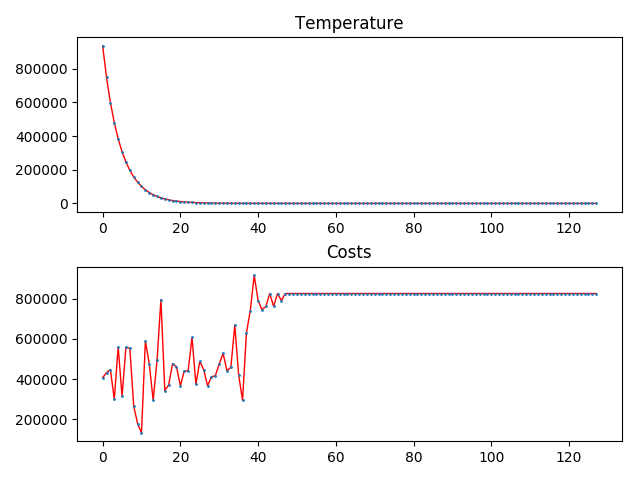
\includegraphics[width=1\linewidth]{results/cut9/2/plot}
  \label{fig:sub1}
\end{subfigure}%
\begin{subfigure}{.5\textwidth}
  \centering
  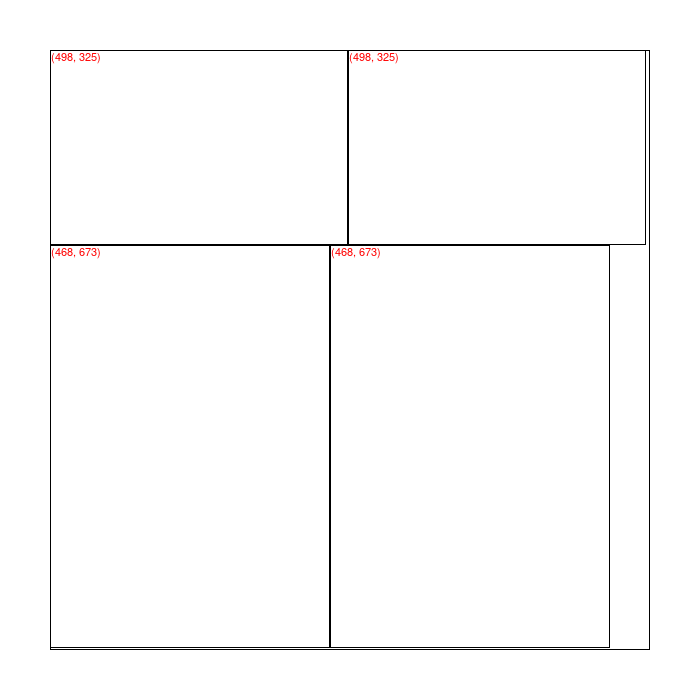
\includegraphics[width=1\linewidth]{results/cut9/2/cut}
  \label{fig:sub2}
\end{subfigure}
\caption{Instancia cut9.txt, Solução: 953628, disperdício de 4.64\% de 1000x1000}
\label{fig:test}
\end{figure}


\begin{figure}
\centering
\begin{subfigure}{.5\textwidth}
  \centering
  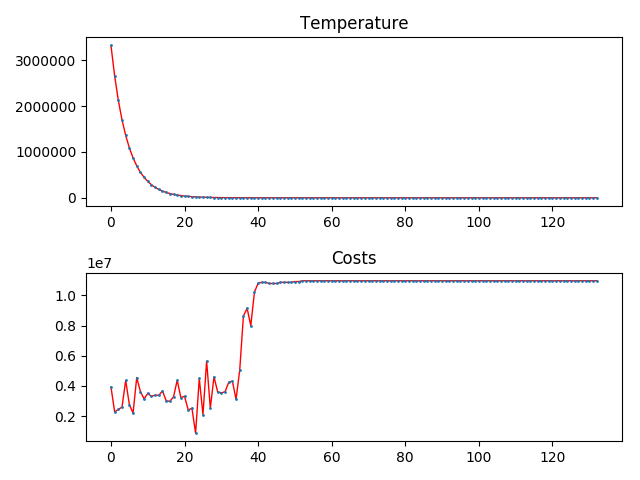
\includegraphics[width=1\linewidth]{results/livre/1/plot}
  \label{fig:sub1}
\end{subfigure}%
\begin{subfigure}{.5\textwidth}
  \centering
  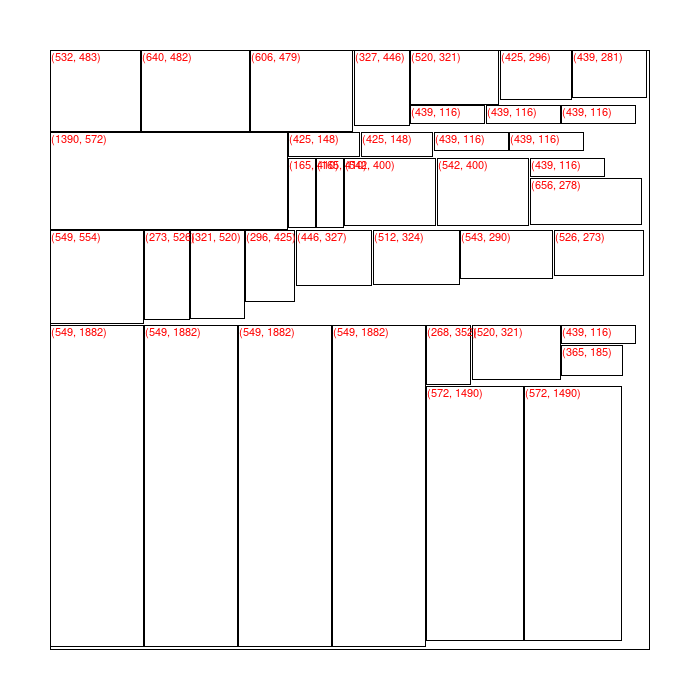
\includegraphics[width=1\linewidth]{results/livre/1/cut}
  \label{fig:sub2}
\end{subfigure}
\caption{Instancia livre.txt, Solução: 11476695, disperdício de 6.31\% de 3500x3500}
\label{fig:test}
\end{figure}

